\documentclass{oci}
\usepackage[utf8]{inputenc}
\usepackage{lipsum}
\usepackage[spanish]{babel}

\title{La cueva de hielo}

\begin{document}
\maketitle
  Terry es una chica a la que le gustan los desafíos.
% En este momento ella se encuentra participando en una difícil competencia organizada por la Organización Cultural de Internet (OCI).
En este momento ella se encuentra participando en una difícil competencia que consiste en completar complejos laberintos de la cueva de hielo de cierta franquicia de criaturas de bolsillo.

Un laberinto consiste en una grilla de $N\times N$ casillas.
Cada casilla es identificada por sus coordenadas $x$ e $y$ ($0\leq x,y \leq N-1$).
Algunas casillas en el laberinto están vacías mientras que otras pueden contener una roca.
Además dos casillas especiales son identificadas como la casilla inicial y final.
Estas casillas están siempre vacías, es decir, no contienen rocas.


El objetivo es mover a un personaje por el laberinto llevándolo desde la casilla inicial hasta la final.
Cada vez que el personaje se mueve a una casilla contigua tarda una unidad de tiempo.
Lo complejo de los laberintos es que el piso es de hielo y por lo tanto el personaje no puede moverse de cualquier forma.
Cada vez que el personaje comienza a moverse en una dirección debe continuar moviéndose en esa dirección hasta chocar con una roca o con el borde del laberinto.
Notar que no basta con que el personaje pase por sobre la casilla final, éste tiene que quedar detenido en esa posición.

La figura de más abajo muestra un laberinto y un posible camino.
El personaje comienza en la casilla $(0, 2)$ y el objetivo es llevarlo a la casilla $(5,1)$.
En primer lugar, el personaje se mueve hacia la derecha hasta chocar con la piedra en la casilla $(4,2)$ quedando detenido en la casilla $(3,2)$.
Este movimiento tarda 3 unidades de tiempo.
A continuación se mueve hacia arriba hasta chocar con el borde superior quedando detenido en la casilla $(3,0)$ y tardando 2 unidades de tiempo.
Los siguientes movimientos llevan al personaje a las casillas $(2,0), (2,3), (1,3), (1,1)$ y finalmente a la casilla $(5,1)$.
El tiempo total ocupado en estos movimientos es $3+2+1+3+1+2+4=16$.

\begin{center}
	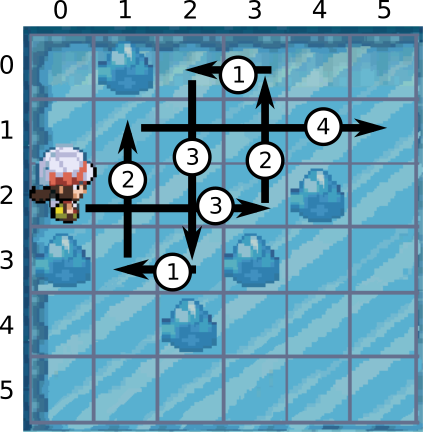
\includegraphics[width=0.4\textwidth]{Icepath2-arrows.png}
\end{center}

\newpage
Terry es una chica muy hábil, pero siempre está ocupada organizando eventos y esta vez no ha tenido tiempo de entrenar para resolver los laberintos.
Terry siempre está disponible para ayudar a quién lo necesite.
Ahora es momento de que tú la ayudes resolviendo estos laberintos.

\subsection*{Subtarea 1 (50pts)}
La primera subtarea consiste en determinar si es posible llevar al personaje desde la casilla inicial a la final.
En esta subtarea no es importante el tiempo que toma mover al personaje.

\begin{itemize}
	\item \verb+bool posible(int N, bool rocas[100][100], int xi, int yi, int xf, int yf)+

  \begin{itemize}
    \item \verb+N+: tamaño de la grilla.
    \item \verb+rocas+: arreglo de dos dimensiones especificando las casillas del laberinto que contienen una roca.
      Si \verb+rocas[x][y]+ guarda el valor \verb+true+ significa que hay una roca en la casilla $(x,y)$, en caso contrario significa que la casilla está vacía.
      Este arreglo es de tamaño $100\times 100$, pero solo las posiciones correspondientes a las primeras $N\times N$ casillas tienen información relevante.
    \item \verb+xi+: coordenada $x$ de la posición inicial.
    \item \verb+yi+: coordenada $y$ de la posición inicial.
    \item \verb+xf+: coordenada $x$ de la posición final.
    \item \verb+yf+: coordenada $y$ de la posición final.
    \item \verb+return+:
      La función debe retornar \verb+true+ si es posible para el laberinto especificado llevar al personaje desde la posición inicial a la final.
      En caso contrario debe retornar \verb+false+.
  \end{itemize}
\end{itemize}
\vspace{-0.6em}

{\bf Restricciones}
\vspace{-1em}
\begin{itemize}
\item Para esta subtarea se probará la función con varios casos donde $10 \leq N\leq 100$ (50pts).
\end{itemize}

\subsection*{Subtarea 2 (50pts)}
En esta subtarea debe encontrarse el mínimo tiempo en que es posible llevar al personaje desde la posición inicial a la final.

\begin{itemize}
	\item \verb+int minimo(int N, bool rocas[100][100], int xi, int yi, int xf, int yf)+

	Esta función debe retornar un entero correspondiente a la mínima cantidad de tiempo en que es posible llevar al personaje desde la posición inicial a la final.
  En caso de no ser posible la función debe retornar $-1$.
  Los parámetros de la función son los mismos que los de \verb+posible+.
\end{itemize}
\vspace{-0.55em}
{\bf Restricciones}
\vspace{-1em}
\begin{itemize}
\item Para esta subtarea se probará la función con varios casos donde $10 \leq N\leq 100$ (50pts).
\end{itemize}

\subsection*{Detalles de implementación}
Debes enviar exactamente un archivo, llamado \verb+hielo.cpp+.
Este archivo debe contener todas las funciones descritas.
Si solo has implementado una de las funciones la otra debe también estar presente y puedes dejarla vacía.
El archivo \verb+hielo.cpp+ debe incluir el header \verb+hielo.h+.

\subsection*{Grader de Ejemplo}
Se provee un \emph{grader} junto con algunos archivos de prueba para que puedas testear tu solución.
El grader lee de la entrada estándar en el siguiente formato.

La primera línea contiene dos enteros $T$ y $N$ correspondientes a la subtarea que se quiere resolver y el tamaño de la grilla.
El número $T$ puede ser 1 o 2.
La siguiente linea contiene cuatro enteros $xi$, $yi$, $xf$ y $yf$.
Correspondientes a las coordenadas de la casilla inicial y la final.
Las siguientes $N$ líneas contienen la descripción de las posiciones de las rocas en la grilla.
Cada línea contiene $N$ enteros separados por espacio.
Estos enteros pueden ser 0 o 1.
Un valor igual a 0 significa que la casilla no contiene una roca y un valor igual a 1 significa que la casilla si contiene una roca.
La coordenada $x$ es numerada de izquierda a derecha y la coordenada $y$ de arriba hacia abajo como se ilustra en la figura de ejemplo mostrada al principio.


\end{document}

%  LocalWords:  Terry